\documentclass[a4paper,10pt]{article}
\usepackage[utf8]{inputenc}
\DeclareUnicodeCharacter{2010}{-}% support older LaTeX versions
\usepackage{hyperref}
\usepackage{amsmath}
\usepackage{tikz}
\usepackage{tikz-qtree}
%\usepackage{subfigure}
\usepackage{graphicx}
\usepackage[numbers]{natbib}

% paper1
\usepackage{amsthm,amssymb,amsfonts}
\usepackage{xspace}
\usepackage{enumitem}
\usepackage{algorithm}
\usepackage{algorithmicx}
\usepackage[noend]{algpseudocode}
\usepackage{algpseudocode}
\usepackage{parskip}
\usepackage{subcaption}
%\usepackage{subfig}

\graphicspath{
	{./figs/}
}

\hypersetup{}
\DeclareMathOperator*{\argmax}{arg\,max}

%opening
\title{Provably Constant-time Motion Planning}
\author{Fahad Islam\\
The Robotics Institute\\
Carnegie Mellon University\\
\texttt{fi@andrew.cmu.edu}}

\newtheorem{theorem}{Theorem}
\newtheorem{lemma}{Lemma}
%\newtheorem{definition}{Definition}
%\newtheorem{cor}{Corollary}

%\newcommand{\calX}{\ensuremath{\mathcal{X}}\xspace}
%\newcommand{\calL}{\ensuremath{\mathcal{L}}\xspace}
%\newcommand{\calS}{\ensuremath{\mathcal{S}}\xspace}
%\newcommand{\calR}{\ensuremath{\mathcal{R}}\xspace}
%\newcommand{\calD}{\ensuremath{\mathcal{D}}\xspace}
%\newcommand{\calP}{\ensuremath{\mathcal{P}}\xspace}

\newcommand{\sAttract}{\ensuremath{s^{\text{attractor}}_i}\xspace}
\newcommand{\sStart}{\ensuremath{s_{\text{start}}\xspace}}
\newcommand{\sGoal}{\ensuremath{s_{\text{goal}}\xspace}}
\newcommand{\sNom}{\ensuremath{s_{\text{nominal}}\xspace}}
\DeclareMathOperator*{\argmin}{arg\,min}
\input{macros2.tex}
\begin{document}

\maketitle

\begin{center}
\Large{Thesis Proposal}
\vspace{40mm}

\large{
\textbf{Thesis Committee:}

Maxim Likhachev (Chair)\\
Chris Atkeson\\
Oliver Kroemer\\
Siddhartha Srinivasa (UW)\\
Oren Salzman (Technion)\\
}
\end{center}
\newpage

\begin{abstract}
In manufacturing and warehouse scenarios, robots often perform recurring manipulation tasks in structured environments. Fast and reliable motion planning is one of the key elements that ensure efficient operations in such environments. A very common example scenario is of manipulators working at conveyor belts, where they have limited time to pick moving objects and if the planner exceeds a certain time threshold, they would fail to pick the objects up. Similar scenarios are encountered in automated assembly lines. Such time-critical applications spur the need for planners which are \emph{guaranteed} to be fast. To this end we introduce the concept of Constant-time Motion Planning (CTMP); namely, the ability to provably guarantee to generate a full motion plan within a (small) constant time. We then develop several algorithms that fall into the class of constant-time motion planning algorithms.

Specifically, up to now we have developed constant-time motion planning algorithms for two domains; (1) Manipulation for repetitive tasks in static environments (2) Manipulation for the task of picking up moving objects (of known models) off a conveyor belt. For the latter, the robot typically perceives a rough pose estimate viewing from a distance, but it must start moving early on (relying on that rough estimate) to be able to reach the object in time and then adjust its motion in real time as it gets improved estimates.
Our key insight is that since these domains are fairly repetitive, the space in which the robot operates is a very small subset of its configuration space, which allows us to preprocess it exhaustively. The preprocessing step generates a representative set of paths that can be used by search at query time in a way that assures small constant-time planning.
%
For the former domain, we evaluate our algorithm for a mail sorting task in simulation on PR2 and also tested the algorithm on a real truck-unloading robot. For the latter domain, we perform real robot experiments on PR2 working at a conveyor belt.

For the remainder of this thesis, we propose to further study and formally define what constant-time planning implies in practice and what underlying assumptions it entails. We also propose to boost the capability of the conveyor pick-up task by having multiple robot arms simultaneously picking up objects, while still maintaining strong theoretical guarantees on the planning side. This introduces new algorithmic challenges including decision making about which object to assign to which arm and motion synchronization between the arms.
\end{abstract}
\newpage

\tableofcontents
\newpage

\section{Introduction}
\subsection{Motivation}
In industrial settings such as manufacturing and warehouse environments, the robots typically operate in structured environments and perform repetitive tasks. Despite significant advancements in the field of motion planning in the past several decades, a large percentage of warehousing and manufacturing industry still uses robots that run hardcoded routines to perform very specific tasks. The lack of penetration of modern motion planning algorithms at scale can be attributed to the fact that the industry needs systems which are \emph{guaranteed} to be fast and reliable, even at the cost of flexibility that these systems could potentially provide.

In warehouses, robots are widely deployed at fast moving conveyor belts to perform repetitive pick and place or sorting tasks, which gives them a very short time buffer to plan their motion. Failing to plan within that time, the robot would skip objects and affect the throughput of the system. Similarly in assembly lines where multiple robots operate in their respective work stations, an overhead caused by the motion planner at one station can slow down the entire chain. This thesis focuses on such time critical applications and introduces the notion of (small) Constant-time Motion Planning (CTMP). CTMP implies generating full motion plans in provably-bounded short planning times.

This thesis is motivated by the following key observations from the aforementioned domains; (1) The tasks are highly repetitious (2) The  environments are fairly structured. (1) gives us an insight that the operational space of the robot is a very small as compared to its full C-space and (2) implies that the environment model is known in advance. These two aspects allow us to fully preprocess the part of the C-space that the robot operates in while accounting for the known objects that exists in its surroundings.

A naive way of providing constant-time guarantees would be to precompute paths for all possible start and goal states that the planner could be queried for and use a simple hash lookup at query time (assuming the lookup time is constant). However, as the set of start or goal states increase, this approach quickly becomes intractable memory and precomputation time wise. Our method provides a compression scheme and precomputes only a small set of representative paths which can still ``cover" the robot's operational space. Namely, using this set of paths, at query time, our method can solve any query within the robot's operational space in bounded time.

\subsection{Approach}
\label{sec:approach}
So far, we have developed CTMP algorithms for two domains.
\subsubsection{Manipulation for repetitive tasks in static environments}
In this work, we consider the specific case where the start state is fixed and there exists a ``goal region" which contains all possible goals. Consider for example, a typical mailroom scenario where the robot has to pick up mail from a fixed location and sort them in cubby shelves. The start corresponds to the pickup location for the packages and the goal region corresponds to all possible goal poses within the cubby shelves. Note that the cubbies reduce the robot's operational space drastically which makes the preprocessing tractable for our method.

Our key insight is that given an ``attractor state''~$s$ in the goal region, typically there is a large region of states around it for which a greedy search (a search following a potential function) towards~$s$ is collision free. We show that such so called attractor regions can be efficiently computed by using dynamic programming.
Importantly, the runtime-complexity of such a greedy search is bounded and there is no need to perform computationally-complex collision-detection operations. 
This insight allows us to generate in an offline phase a small set of these attractor regions together with a path between each attractor state and the start, ensuring that together these attractor regions completely cover the full goal region.
In the query phase, a path is generated by performing a greedy search from the goal to an attractor state (the one which contains the goal) followed by the precomputed path from the start.

\subsubsection{Manipulation for picking up moving objects off a conveyor belt}
We will refer to this problem as ``conveyor pickup task". For this domain we assume that the geometric models of the target objects are known in advance. The success of manipulation tasks relies heavily on the accuracy of the perception system which often is noisy, especially if the target objects are perceived from a distance. For fast moving conveyor belts, the robot cannot wait for a perfect estimate before it starts execution. In order to be able to reach the object in time it must start moving early on (relying on the initial noisy estimates) and adjust its motion on-the-fly in response to the pose updates from perception. We developed an approach that meets these requirements by providing provable constant-time planning and replanning guarantees.

Again, with the same insight, in the first step we precompute a small set of paths from a fixed start (say drop off location) that can cover the goal region which in this domain is defined in the space of object poses. The goal can be any arbitrary object pose~$(x,y,yaw)$ of the objects. In the second step, we uniformly discretize these paths in time to get a set of states that we call ``replannable'' states. To handle pose updates online, we may need to replan from any of these states to all the goals in the goal region. The algorithm then goes back to the first step treating all the replannable states as new starts and this recursive process continues until all replannable states are taken care of. While the approach has exponential complexity in the number of timesteps from the start to the goal, we drastically save on computation and memory by reusing the first set of paths (from the drop off location to the goal region). Our algorithm guarantees that for any replannable state and a goal, a plan will be generated within a bounded time. Experimentally we observe that the robot fails most of the time without replanning i.e. in case it relies on the first estimate or if it waits for an accurate estimate before starting planning.

\subsection{Expected Contribution}
We expect to make the following contributions in this thesis.
\begin{itemize}
	\item Introduce and formalize the concept of Constant-time Motion Planning (CTMP)
	\item Develop CTMP algorithm for domains with repetitive manipulation tasks in static environments
	\item Develop CTMP algorithm for the conveyor pickup task
	\item Enhance the conveyor pick task using multiple robot arms, simultaneously picking up multiple objects
\end{itemize}

\section{Background}
\subsection{Configuration Space and Motion Planning}
Motion planning algorithms operate in the state space often also referred to as the \emph{configuration space} (C-space) or~$\calC$~\cite{lozano1990spatial}. In this space a state or a configuration of the robot can be uniquely represented as a point which makes it convenient for the motion planners to operate. It can be the~($x,y$) position of the robot or~($x,y,yaw$) if the orientation also matters. For a robot arm the configuration can be composed of all the joint positions. If planning with dynamics, the velocities and times may also be added to the configuration. Similarly higher order derivatives can also be added as per the requirements of the domain. The number of variables in the configuration represents the \emph{dimension} of the C-space. For example, for a 7DoF robot arm, for only considering the joint positions, the dimension of the C-space is seven. The free space~$\Cfree$ contains all the configurations which are valid with respect to some state validity criterion such as violation of obstacle collision constraints or kinematic constraints etc. The obstacle space~$\Cobs$ contains all the configurations which are invalid and so~$\Cobs = \calC \backslash \Cfree$

For the motion planning problem we define a start configuration~$\Sstart$ and a goal set~$\Sgoal$. The goal can be under-specified as the pose of the robot end-effector or the pose of the target object. For instance, given a target object that the robot needs to grasp, the goal can be the grasp pose (i.e. position and orientation of the end-effector) or it can be even more under-specified as the pose of the object, giving the flexiblity to select different grasp poses. The motion planning problem is defined as finding a continuous path~$\tau : [0:1] \rightarrow \Cfree$ s.t. $\tau(0) = \Sstart$ and $\tau(1) \in \Sgoal $. Typically in practice most motion planning algorithms find a path of the form~$[s_0, s_1, s_2,...,s_n] \in \Cfree$ s.t. $s_0 = \Sstart$ and $s_n \in \Sgoal$ assuming that the consecutive states i.e $s_i, s_{i+1}$ can be connected via some simple interpolation scheme.

Computing~$\Cfree$ is extremely hard, specially in higher dimensions. Instead of doing that, most motion planners generally sample in~$\Cfree$ and use a collision checker to identify the validity of a configuration. These planners typically sample states in~$\Cfree$ using rejection sampling, connect those samples to construct a graph (or a tree) and then use graph search to find the path from a start to goal. These algorithms are called sampling-based algorithms. A motion planner is referred to as \emph{complete} if it guarantees to find a path if one exists, and otherwise returns failure. Sampling-based planners are \emph{probablisitically complete}, meaning that in the limit of the number of samples they are guaranteed to find a solution if one exists.

\subsection{C-space representation for Search-based Planning}
\label{sec:sbp}
Search-based planning methods descritize the C-space into cells. This descritization relies generally relies on a grid-based or lattice-based structure. A cell is the smallest unit of this discrete space and represents a small volume of C-space states that lie within it. A representative state within a cell, commonly its geometric center is picked to denote a vertex for that cell. All the vertices~$\calV$ connect to their neighboring vertices through edges~$\calE$ to construct a graph~$\calG = (\calV, \calE)$. These edges may have associated costs. Only those vertices and edges are added to~$\calG$ that are valid. The motion planning problem is thus turned into a graph search problem which can be solved using any graph search algorithim. The search is done on an implicit graph as opposed to explicit graph. Namely, instead of precomputing the entire graph which is infeasible for large domains, the graph is constructed and evaluated on-the-fly as the search progresses.

The C-space discretization is done at a certain resolution which is a domain dependent parameter. The resolution determines how course or fine the discretization is. Search-based algorithms are attributed as \emph{resolution complete} which means that they will return a path if one exists for the given resolution. Note that it is possible that a solution exists in the C-space and the search-based planner fails to find it because the resolution is not fine enough for that problem.

\subsection{Computational Complexity in Motion Planning}
The general motion planning problem was shown by Reif to be PSPACE-hard~\cite{reif1979complexity}. Later it was shown to be PSPACE-complete by Canny~\cite{canny1988complexity}. Their analysis was based on finding the \emph{exact} solutions. The class of algorithms that go for finding the exact solutions are called combinatorial algorithms or \emph{exact} algorithms~\cite{lavalle2006planning}. These algorithms do not rely on any approximation of the C-space and operate in the continuous C-space. They are also complete with respect to the continuous C-space which is a stronger notion of completeness compared to sampling-based planners or search-based planners which are probablisitically complete and resolution complete respectively.

The dimension~$d$ of the C-space is the most crucial element in determining the complexity of the motion planning problem. It has been shown that for the general motion planning problem the computational complexity grows exponentially with~$d$~\cite{chazelle1991singly}.

The exact motion planning algorithms do not scale to more complex problems as they make certain limiting assumptions about the geometry of the robot and the obstacles. Since the exact methods are no more used in modern days, the computational complexity analysis for the general motion planning problem is of less relevance and the community focusses more on the analysis of the specific algorithms.



\section{Related Work}
\subsection{Preprocessing-based Methods}
Preprocessing-based motion planners often prove beneficial for real-time planning. They analyse the configuration space offline to generate some auxiliary information that can be used online to speed up planning. 

The most reknowned example is the Probablistic Roadmap Method (PRM)~\cite{kavraki1996probabilistic} methods. They have a preprocessing and a query phase. In the preprocessing phase a roadmap is constructed in $\Cfree$ by randomly sampling valid states in the C-space and connecting them to their neighboring states if the edges making the connections are valid. In the query phase the start and goal states are connected to their neighboring states in the roadmap (if valid connections are possible) and then any search algorithm like A* search is used to find the path. PRM methods are categorized as multi-query methods meaning that once the roadmap is constructed it can be used to answer multiple queries for the same environment. Query times can be significantly sped up by further preprocessing the roadmaps using landmarks~\cite{paden2017landmark}. Recently,the repetition roadmap~\cite{LA18} was suggested as a way to extend the \textsf{PRM} for the case of multiple highly-similar scenarios. Some of these methods have been integrated with sparse motion-planning roadmaps (see e.g.,~\cite{SSAH14,DB14}) to reduce the memory footprint of the algorithm. All these methods only provide probablistic completeness guarantees.

Our work bares resemblance to previous work on 
subgoal graphs~\cite{UK17,UK18}.
Subgoal graphs is a search-based method that preprocesses the entire C-space to generate a sparse overlay graph comprised of vertices called sub-goals. The pair of sub-goals connected by an edge are \emph{reachable} and thus searching on this overlay graph is significantly faster than searching on the original graph. The method assures that the path found on this subgoal graph has a path on the original graph and can be quickly computed at query time. As this method requires preprocessing the full C-space it is expensive and only is applicable to lower dimensional planning problems.

While all these preprocessing-based approaches speedup planning times compared to planning from scratch by using the preprocessed information, they do not provide bounds on the planning times.


\subsection{Motion Planning with Reuse}
An alternative approach to address our problem is to precompute a set of complete paths into a library and given a query, attempt to match complete paths from the library to the new query~\cite{berenson2012robot,jetchev2013fast}.
Using paths from previous search episodes (also known as using experience) has also been an active line of work~\cite{PCCL12,PDCL13,BAG12,CSMOC15}. E-graphs method~\cite{PCCL12} computes a heuristic function to guide the search in such a way as to reuse search efforts from previously generated paths. The Lightning framework~\cite{BAG12} runs two modules in parallel, a module that runs the planner from scratch and a module that retrieves and repairs path stored in a library. The Thunder framework~\cite{CSMOC15} also leverages previous experiences and the experiences are generated using probabilistic sampling. The experiences as stored as sparse roadmap spanner~(SPARS). 

These methods also provide significant speedups in planning times, but they still do not provide constant-time planning guarantees which our method aims to provide.

\subsection{Real-time Motion Planning}
In practice, the only class of algorithms that provide constant-time planning guarantees are real-time algorithms~\cite{KL06,KS09,K90}.
To provide guarantees on planning time the search only looks at a finite horizon, generating a partial plan, and interleaves planning and execution. These algorithms run repeated A* searches and update the heuristic values in the local search spaces while maintaining the admissibility of the heuristics. The heuristis get more informed as the search is run repeatedly. By doing so they provide completeness guarantees, meaning that the robot will eventually arrive at the goal.

As opposed to these finite horizon planning algorithms, our method plans for indefinite horizons i.e. all the way from the start to the goal while providing constant-time planning guarantees

\subsection{Online Replanning: Moving Target Search}
The conveyor-planning problem can be modelled as a Moving Target Search problem (MTS) which is a widely-studied topic in the graph search-based planning literature~\cite{ishida1991moving,ishida1995moving,koenig2007speeding,sun2010moving}. 
These approaches interleave planning and execution incrementally and update the heuristic values of the state space to improve the distance estimates to the moving target. Unfortunately, in high-dimensional planning problems, this process is computationally expensive which is why these approaches are typically used for two-dimensional grid problem such as those encountered in video games.

\subsection{Global Control using Local Potential Functions}
Finally, our notion of attractor states is similar (in spirit) to control-based methods that  ensure safe operation over local regions of the free configuration space~\cite{CRC03,CCR06,tedrake2010lqr}. Metaphorically they name these regions as ``funnels" that collapse a large set of input conditions to a single policy,
These regions are then used within a high-level motion planner to compute collision-free paths. LQR-trees~\cite{tedrake2010lqr} computes local stability regions to build a sparse tree of LQR-stabilized trajectories. The union of these local regions covers the entire state space.

\subsection{Motion Planning for Conveyor Pickup Task}
Existing work on picking moving objects has focused on different aspects of the problem ranging from closed-loop controls to object perception and pose estimation, motion planning and others~\cite{allen1993automated, han2019toward, stogl2017tracking, zhang2018gilbreth}. 
%
Here, we focus on motion-planning related work. Graph-searched based approaches have been used for the motion-planning problem~\cite{cowley2013perception, menon2014motion}. The former uses a kinodynamic motion planner to smoothly pick up moving objects i.e., without an impactful contact. A heuristic search-based motion planner that plans with dynamics and could generate optimal trajectories with respect to the time of execution was used. While this planner provides strong optimality guarantees, it is not real-time and thus cannot be used online.
%
The latter work was demonstrated in the real world showing real-time planning capability. While the planner is fast, it does  pure kinematic planning and does not require collision checking with the target object. The approach plans to a pregrasp pose and relies on Cartesian-space controllers to perform the pick up. The usage of the Cartesian controller limits the types of objects that the robot can grasp.

\section{Constant-time Motion Planning (CTMP)}
\label{sec:ctmp}
In this thesis we introduce the concept of Constant-time Motion Planning (CTMP). We develop algorithms that will provably guarantee constant query-time complexity. Constant-time complexity implies that regardless of the problem size or the input size, the algorithm demands the same computation time.

\subsection{Input size of the Algorithm}
As described in section~\ref{sec:conveyor}, our approach operates in discretized search spaces. The size of the input to the query phase of our algorithm is determined by the size of the discretized operational space of the robot. 
To prove that the algorithm has a constant time complexity, we need to show that its computation time is bounded and the bound is independent of the input size.
%In our problem setting our input to the algorithm is the full configuration space of the robot~$\calC$. The size of~$\calC$ by definition is unbounded since it is a continuous space. We will also consider the case in section~\ref{sec:conveyor} where we consider a discretized search space as highlighted in section~\ref{sec:sbp}. In that case the input is finite is defined by the size of the underlying implicit graph~$\calG$. 

\subsection{(Small) Constant-time Algorithm}
More formally an algorithm with input size~$n$ has a constant time complexity if~$T(n)$ is bounded by a value that does not depend on~$n$.
Note that the running time does not have to be independent of~$n$, but an upper bound for the running time has to be bounded independently of~$n$. In Big O notation, a constant-time algorithm has an asymptotic complexity of~$O(1)$. In the proposed constant-time algorithms we also aim that~$T(n)$ of the algorithm is small as to have real-time performance.

\subsubsection{A Naive Constant-time Algorithm}
Refering to the problem setting described in section~\ref{sec:approach}, given a goal region~$G$ with a finite set of goals, the naive approach would be to precompute and store paths to each goal in~$G$ in a preprocessing stage and use a hash table mapping goals to paths and use it to answer any query goal~$g \in G$ in the query stage. Under the assumption that there are no hash collisions, the hash lookup is considered a constant-time operation and hence the algorithm will have a constant-time complexity. However, this approach becomes intractable when the number of queries becomes large. This is because the memory requirement or the precomputation time becomes very large for computational resources.

\subsubsection{Proposed Approach}
The naive approach puts all the computation burden on the proprocessing phase and requires minimum computation time but a large memory during the query phase. On the other end of the spectrum we can just plan from scratch online every time and eliminate the preprocessing stage, shifting all the burden to the query phase. This would require minimal memory but the high computational complexity. We propose a middle ground where we can balance the offline-online burden in such a way that we can provide provable (small) constant time planning guarantees. Instead of having to precompute paths to all the goals in~$G$, we propose compression schemes to precompute and store only a small set of representative paths that can be used in query phase in such a way that assures (small) constant time planning. In the following two sections we will theoretically show that our algorithms run in constant-time and experimentally show that the planning times are small.


\section{CTMP for Repetitive Tasks in Static Environments}
\subsection{Algorithm Framework}
\label{sec:alg}
In this section we describe our algorithmic framework. We start (Sec.~\ref{sec:pdef}) by formally defining our problem and continue (Sec.~\ref{sec:key}) by describing the key idea that enables our approach.
We then proceed (Sec.~\ref{subsec:alg}) to detail our algorithm and conclude with implementation details (Sec.~\ref{subsec:impl}).

\subsubsection{Problem formulation and assumptions}
\label{sec:pdef}
Let $\calX$ be the configuration space of a robot operating in a static environment containing obstacles.
We say that a configuration is valid (invalid) if the robot, placed in that configuration does not (does) collide with obstacles, respectively.
We are given in advance a start configuration~$\Sstart \in \calX$ and some goal region~$G \subset \calX$.
We emphasize that the goal region may contain invalid configurations.
In the query phase we are given multiple queries $(\Sstart, s_{\text{goal}})$ where $s_{\rm goal} \in G$ is a valid configuration and for each query, we need to compute a collision-free path connecting $\Sstart$ to $s_{\text{goal}}$.

Coming back to our motivating example of mail sorting---the start configuration would be some predefined configuration above the cart where the robot can pick up the envelopes from and the goal region would comprise of all possible placements of the robot's end effector in the cubbies. The environment is static as the only obstacles in the environment are the shelves and the cart which remain stationary in between queries.

We discretize $\calX$ into a state lattice $\calS$ such that any state~$s \in \calS$ is connected to a set of successors and predecessors via a mapping Succs/Preds: $\calS \rightarrow 2^\calS$.
Define $G_\calS := \calS \cap G$ to be the states that reside in the goal region. Note that although our approach is applicable to general graphs (directed or undirected), to be able to reuse the planned path in the reverse direction (e.g. in our motivating example for the motion from the shelve to the start configuration) the graph needs to be undirected.
We make the following assumptions:

\begin{enumerate}[label={\textbf{A\arabic*}}]
  \item \label{assum:1} $G_\calS$ is a relatively small subset of $S$. Namely, it is feasible to exhaustively iterate over all states in $G_\calS$.
However, storing a path from $\Sstart$ to each state in $G_\calS$ is infeasible.
  
  \item \label{assum:2} The planner has access to a heuristic function $h: \calS \times \calS \rightarrow \mathbb{R}$ which can estimate the distance between any two states in $G_\calS$. Moreover, 
 \begin{itemize}
  \item The heuristic function should be \textit{weakly-monotone} with respect to $G_\calS$, meaning that $\forall s_1, s_2  \in G_\calS$ where $s_1 \neq s_2 $, it holds that,
  \begin{center}
    $h(s_1, s_2) \geq \min\limits_{s_1' \in \text{Preds}(s_1)} h(s_1', s_2)$.
  \end{center}

  \item The heuristic function $h$ should induce that the goal region is \emph{convex} with respect to $h$, meaning that $\forall s_1, s_2  \in G_\calS$ where $s_1 \neq s_2 $, it holds that,
  \begin{center}
     $\argmin\limits_{s_1' \in \text{Preds}(s_1)} h(s_1', s_2) \in G_\calS$.
  \end{center}

 \end{itemize}
 Namely, for any distinct pair of states ($s_1, s_2$) in $G_\calS$, at least one of $s_1$'s predecessors has a heuristic value less than or equal to its heuristic value.
 Moreover, the predecessor with minimal heuristic value lies in the goal region.


  \item \label{assum:3} The planner has access to a tie-breaking rule that can be used to define a total order \footnote{A total order is a binary relation on some set which is anti-symmetric, transitive, and a convex relation.} over all states with the same heuristic value.
  % to a given state.
  \end{enumerate}

These assumptions allow us to establish strong theoretical properties regarding the efficiency of our planner. Namely, that
within a known bounded time, we can compute a collision-free path from $\Sstart$ to any state in $G_\calS$. 


Assumption~\ref{assum:2} may seem too restrictive (especially convexity), imposing that the goal region cannot be of arbitrary structure. However, after we detail our algorithm (Sec.~\ref{subsec:alg}) and analyze its theoretical properties (Sec.~\ref{sec:analysis}), we sketch how we can relax this assumption to be less restrictive.


 
\subsubsection{Key idea}
\label{sec:key}
Our algorithm relies heavily on the notion of a greedy search.  Thus, before we describe of our algorithm, we formally define the terms greedy predecessor and greedy search.

\vspace{2mm}
\begin{definition}
\label{def:greedy-suc}
  Let $s$ be some state and $h(\cdot)$ be some heuristic function.
  A state $s' \in \text{Preds}(s)$ is said to be a \emph{greedy} predecessor of $s$ according to $h$ if it has the minimal $h$-value among all of $s$'s predecessors.
\end{definition}
Note that 
if $h$ is weakly monotone with respect to $G_\calS$
(Assumption~\ref{assum:2}) 
and we have some tie-breaking rule
(Assumption~\ref{assum:3}), then every state has a greedy predecessor in the $G_\calS$ and it is unique.
In the rest of the text, when we use the term greedy predecessor, we assume that it is unique and in $G_\calS$.

\vspace{2mm}
\begin{definition}
  Given a heuristic function $h(\cdot)$,
  an algorithm is said to be a \emph{greedy search}  with respect to $h$ if for every state it returns its greedy predecessor according to $h$.
\end{definition}
Note that we define the greedy search in terms of the predecessors and not the successors to account for the directionality of the graph. This will become more clear in Sec.~\ref{subsec:alg}.

\textbf{Remark:} Now that we have the notion of greedy search, we can better explain our definition of convexity with respect to~$h$ (Assumption~\ref{assum:2});
this assumption ensures that a greedy search between any pair of states lies within the goal region, analogously to the standard notion of a convex region where for every pair of points within the region, every point on the straight line segment that joins the pair of points is also within the region.

Our key insight is to precompute in an offline phase subregions within the goal region where a greedy search to a certain (``attractor'') state is guaranteed to be collision free and use these subregions in the query phase.
Specifically, in the preprocessing phase, $G_\calS$ is decomposed into a finite  set of (possibly overlapping) subregions $\calR$.
Each subregion $R_i \in \calR$ is a hyper-ball defined using a center which we refer to as the ``attractor state''~
\sAttract and a radius $r_i$.
These subregions, which may contain invalid states, are constructed in such a way that the following two properties hold
\begin{enumerate}[label={\textbf{P\arabic*}}]
  \item \label{property:1} For any valid goal state $s_{\text{goal}} \in R_i \cap G_\calS$, a greedy search with respect to $h(s, \sAttract)$ over $\calS$ starting at $\sGoal$ will result in a collision-free path to \sAttract.
  \item \label{property:2} The union of all the subregions completely cover the valid states in $G_\calS$. 
      Namely, $\forall s \in G_\calS~\text{s.t.}~s~\text{is valid}, \exists R \in \calR \ s.t. \ s \in R$.
\end{enumerate}

In the preprocessing stage, we precompute a library of collision-free paths $\calL$ which includes a path from $\Sstart$ to each attractor state. 
In the query phase, given a query~\sGoal, we 
(i)~identify a subregion $R_i$ such that $\sGoal \in R_i$ (using the precomputed radii~$r_i$),
(ii)~run a greedy search towards~\sAttract by greedily choosing at every point the predecessor that minimizes~$h$ and
(iii)~append this path with the precomputed path in $\calL$ to $\Sstart$ to obtain the complete plan.
For a visualization of our algorithm, see Fig.~\ref{fig:approach}.


\begin{figure}
\centering
\includegraphics[width=0.45\textwidth]{approach.pdf}
    % \vspace{-2mm}
  \caption{
  Visualization of approach. Subregions are depicted in green, 
  goal region~$G$ is depicted in tiled gray  containing obstacles (red).
  Precomputed paths from $s_{\rm{start}}$ to attractor states are depicted in blue.
 Given a query $(s_{\rm{start}}, s_{\rm{goal}})$, the returned path is given by $\pi_i$ appended with a greedy path ~$\pi_g$ from $s_{\rm{goal}}$ to \sAttract (reversed), which is depicted in purple.
}
    \label{fig:approach}
% \vspace{-6mm}
\end{figure}

\subsection {Algorithm}
\label{subsec:alg}
\subsubsection{Preprocessing Phase}
The preprocessing phase of our algorithm, detailed in Alg.~\ref{alg:1}, takes as input the start state~$\Sstart$, the goal region~$G_\calS$ and a conventional motion planner $\calP$, and outputs a set of subregions~$\calR$ and the corresponding library of paths~$\calL$ from~\Sstart to each~\sAttract. 

The algorithm covers~$G_\calS$ by iteratively finding a state $s$ not covered\footnote{Here, a state $s$ is said to be covered if there exists some subregion $R \in \calR$ such that $s \in R$.} by any subregion and computing a new subregion centered at $s$.
To ensure that $G_\calS$ is completely covered (Property~\ref{property:2}) we maintain a set~$V$ of valid (collision free) and a set $I$ of invalid (in collision) states called \emph{frontier states} (lines~\ref{alg:1:v} and~\ref{alg:1:i}, respectively).
We also construct subregions centered around invalid states~$\hat{\calR}$ to efficiently store which invalid states have been considered.
We start by initializing~$V$ with some random state in $G_\calS$ and iterate until both~$V$ and~$I$ are empty, which will ensure that $G_\calS$ is indeed covered even if $G_\calS$ is not fully connected.

At every iteration, we pop a state from $V$ (line~\ref{alg:1:pop}), and if there is no subregion covering it, we add it as a new attractor state and compute a path $\pi_i$ from $\Sstart$ (line~\ref{alg:1:path}) using the planner $\calP$.
We then compute the corresponding subregion (line~\ref{alg:1:cr} and Alg.~\ref{alg:2}).

As we will see shortly, computing a subregion corresponds to a Dijkstra-like search centered at the attractor state.
The search terminates with the subregion's radius $r_i$ and a list of frontier states that comprise of the subregion's boundary.
The valid and invalid frontier states are then added to $V$ and $I$, respectively (lines~\ref{alg:1:insert_v} and~\ref{alg:1:insert_i}).


Once $V$ gets empty the algorithm starts to search for states which are valid and yet uncovered by growing subregions around invalid states popped from~$I$ (lines~\ref{alg:1:iv_loop}-\ref{alg:1:iv_region} and detailed in Alg.~\ref{alg:3b}). If a valid and uncovered state is found, it is added to $V$ and the algorithm goes back to computing subregions centered at valid states (lines~\ref{alg:1:x_states}-\ref{alg:1:break}), otherwise if $I$ also gets empty, the algorithm terminates and it is guaranteed that each valid state contained in $G_\calS$ is covered by at least one subregion.

\begin{algorithm}[t]
\footnotesize
\hspace*{\algorithmicindent} \textbf{Inputs:} $G_\calS$, $\Sstart$, $\calP$
\Comment{goal region, start state and a planner} 

\hspace*{\algorithmicindent} \textbf{Outputs:} 
$\calR, \calL$
%$R_i = (\sAttract, r_i)$, $\pi_i$,
\Comment{subregions and corresponding paths to $\Sstart$}

%\hspace*{\algorithmicindent}
% \textbf{Parameters:} $r_{\text{max}}$   \Comment{maximum radius of a region}
\caption{Goal Region Preprocessing}\label{alg:1}
\begin{algorithmic}[1]
\Procedure{PreprocessRegion}{$G_\calS$}
%\Procedure{PreprocessRegion}{$G, r_{\text{max}}$}
  \State $s \leftarrow$\textsc{ SampleValidState}($G_\calS$)
  \State $V \leftarrow \{ s \}$   \Comment{valid frontier states initialized to random {state}} \label{alg:1:v}
  \State $I$ = $\emptyset$   \Comment{invalid frontier states} \label{alg:1:i}
  \State $ i \leftarrow 0$
       \hspace{2mm} 
       $\calL = \emptyset$
       \hspace{2mm} 
       $\calR = \emptyset$
       \hspace{2mm} 
       $\hat{\calR} = \emptyset$
       
  \vspace{2mm}
    \While {$V$ and $I$ are not empty}
        \While {$V$ is not empty}
          \State $s \leftarrow V.\text{pop}()$ \label{alg:1:pop}
            \If {$\nexists R \in \calR$  s.t. $s \in R$ }  \label{alg:1:discard}
            \Comment{$s$ is not covered}
        \State $\sAttract \leftarrow s$               
        \label{alg:1:attract} 
                \State $\pi_i$ = $\calP.$\textsc{PlanPath}($\Sstart, \sAttract$); \label{alg:1:pp}
                \hspace{2mm }
                $\calL \leftarrow \calL \cup \{ \pi_i \}$  \label{alg:1:path}
                \State $(\text{OPEN}, r_i) \leftarrow$ \textsc{ComputeReachability}($\sAttract$) \label{alg:1:cr}
%                \State $(\text{OPEN}, r_i) \leftarrow$ \textsc{ComputeReachability}($\sAttract, r_{\text{max}}$) \label{alg:1:cr}
                \State insert Valid(OPEN) in $V$  \label{alg:1:insert_v}
                \State insert Invalid(OPEN) in $I$   \label{alg:1:insert_i}
                \State $R_i$ $\leftarrow$ $(\sAttract, r_i)$; 
                \hspace{2mm} $ i \leftarrow i+1$        \hspace{2mm }
                $\calR \leftarrow \calR \cup \{ R_i \}$
                            \EndIf
        \EndWhile

\vspace{2mm}        
        
        \While {$I$ is not empty} \label{alg:1:iv_loop}
            \State $s$ $\leftarrow$ $I.pop()$
      \If {$\nexists R \in \calR \cup \hat{\calR}$ s.t. $s \in R$ }      \Comment{$s$ is not covered}
\State $(X, r)$ $\leftarrow$ \textsc{FindValidUncoveredState}($s$)
%                \State $(X, r)$ $\leftarrow$ \textsc{FindValidUncoveredState}($s, r_{\text{max}}$)
                \State $\hat{R}$ $\leftarrow$ $(s,r)$;
        \hspace{2mm}
        $\hat{\calR} \leftarrow \hat{\calR} \cup \{ \hat{R} \}$ \Comment{invalid subregion}  \label{alg:1:iv_region}
                \If {$X$ is not empty}  \Comment{valid state found}  \label{alg:1:x_states}
                    \State insert $X$ in $V$
                    \State \textbf{break} \label{alg:1:break}
                \EndIf
            \EndIf
        \EndWhile
    \EndWhile

  \vspace{2mm}

  \State \Return $\calR, \calL$
\EndProcedure
\end{algorithmic}
\end{algorithm}

\begin{figure}[tb]
  \centering
    \includegraphics[width=0.3\textwidth]{alg2.pdf}
    % \vspace{-2mm}
  \caption{
  Visualization of Alg~\ref{alg:2}. Subregion $R_i$ (green) grown from $\sAttract$ in a goal region~$G$ (tiled grey) containing an obstacle (red).
  Frontier states and first state not in $R_i$ are depicted by circles and a cross, respectively.
}
    \label{fig:alg2}
% \vspace{-6mm}
\end{figure}

\subsubsection{Reachability Search}
The core of our planner lies in the way we compute the subregions (Alg.~\ref{alg:2} and Fig.~\ref{fig:alg2}) which we call a ``Reachability Search''. The algorithm maintains a set of \emph{reachable} states $S_{\text{reachable}}$ for which Property~\ref{property:1} holds.
As we will see, this will ensure that in the query phase, we can run a greedy search from any reachable state $s \in S_{\text{reachable}}$ and it will terminate in the attractor state. 
%
The following recursive definition formally captures the notion of a reachable state.

\vspace{2mm}
\begin{definition}
  Given some attractor state \sAttract, we say that a state $s \in G_\calS$ is reachable under some function $h(\cdot)$ with respect to \sAttract if either
  (i)~$s = \sAttract$ or
  (ii)~the greedy predecessor of $s$ with respect to $h(s,\sAttract)$ is reachable.
\end{definition}

The algorithm computes a subregion that covers the maximum number of reachable states that can fit into a hyper-ball defined by $h(s,\sAttract)$. 
The search maintains a priority queue OPEN ordered according to $h(s,\sAttract)$. Initially, the successors of $\sAttract$ are inserted in the OPEN (line~\ref{alg:2:OPEN}). For each expanded successor, if its valid greedy predecessor is in $S_{\text{reachable}}$, then the successor is also labeled as reachable (lines~\ref{alg:2:crit} and~\ref{alg:2:set}). 

The algorithm terminates when the search pops a state which is valid but does not have a greedy predecessor state in $S_{\text{reachable}}$ (line~\ref{alg:2:terminate}). Intuitively, this corresponds to  the condition when the reachability search exits an obstacle (see Fig.~\ref{fig:alg2}).
At termination, all the states within the boundary of radius $r_i$ (excluding the boundary) are reachable.


\begin{algorithm}[t]
\footnotesize
\caption{Reachability Search}\label{alg:2}

\begin{algorithmic}[1]
\Procedure{ComputeReachability}{$\sAttract$}
%\Procedure{ComputeReachability}{$\sAttract, r_{\text{max}}$}
\State $S_{\text{reachable}} \leftarrow \{\sAttract\}$ \Comment{reachable set} \label{alg:2:reachable}
\State OPEN $\leftarrow \{$Succs($\sAttract$)$\}$  \Comment{key: $h(s,\sAttract)$} \label{alg:2:OPEN}
\State CLOSED $\leftarrow \emptyset$
\State $r_i \leftarrow 0$

%\While {$r_i \leq r_{\text{max}}$}
\While{OPEN$\neq \emptyset$}
    \State $s \leftarrow$ OPEN.pop()
    \State insert $s$ in CLOSED
    \State $s'_g \leftarrow \argmin\limits_{s' \in \text{Preds}(s)} h(s', \sAttract)$ 
%    \State $s'_g \leftarrow$ GreedySucc($s$)
  \label{alg:2:greedy} 
 \Comment{greedy predecessor}
 % acc. to some tie-breaking criteria}
    \If {$s'_g$ $\in$ $S_{\text{reachable}}$ and Valid(edge(s,$s'_g$))}  \label{alg:2:crit}
        \State $S_{\text{reachable}} \leftarrow S_{\text{reachable}} \cup \{s\}$  \Comment{$s$ is greedy} \label{alg:2:set}
    \ElsIf {Valid($s$)} \label{alg:2:terminate}
        \State $r_i \leftarrow h(s, \sAttract)$ \label{alg:2:rad}
        \State \Return (OPEN, $r_i$)
%        \State break
    \EndIf
    \For {each $s' \in \text{Succs}(s) \cap G_\calS$} \label{alg:2:prun}
        \If {$s' \notin$ CLOSED}
            \State insert $s'$ in OPEN with priority $h(s', \sAttract)$
        \EndIf
    \EndFor
\EndWhile
\State $r_i \leftarrow h(s, \sAttract) + \epsilon$    \Comment{$\epsilon$ is a small positive constant}
\State \Return (OPEN, $r_i$)

\EndProcedure
\end{algorithmic}
\end{algorithm}

\begin{algorithm}[t]
\footnotesize
\caption{Find valid uncovered state}\label{alg:3b}

\begin{algorithmic}[1]
\Procedure{FindValidUncoveredState}{$\hat{s}$}
\State OPEN $\leftarrow \{\hat{s}\}$
\While{OPEN$\neq \emptyset$}
  \State $s \leftarrow$ OPEN.pop()
  \State insert $s$ in CLOSED
  \If {$\nexists R \in \calR$  s.t. $s \in R$ and Valid(s)}
  % \Comment{$s$ is not covered and $s$ is valid}
    \State \Return ($\{s\}$, $h$($s$, $\hat{s}$))
  \EndIf
  \For {each $s' \in \{\text{Succs}(s) \cup \text{Preds}(s)\} \cap G_\calS$}
    \If {$s' \notin$ CLOSED}
        \State insert $s'$ in OPEN with priority $h(s', \sAttract)$
    \EndIf
  \EndFor
\EndWhile
\State $r = h$($s$, $\hat{s})) + \epsilon$    \Comment{$\epsilon$ is a small positive constant}
\State \Return ($\emptyset$, $r$))
\EndProcedure
\end{algorithmic}
\end{algorithm}


\subsubsection{Query Phase}
Given a query goal state $s_{\text{goal}} \in G_\calS$ 
our algorithm, detailed in Alg.~\ref{alg:3}, starts by finding a subregion $R_i \in \calR$ which covers it (line.~\ref{alg:3:covers}). Namely, a subregion~$R_i$ for which 
$h(s_{\text{goal}}, \sAttract) < r_i$.
We then run a greedy search starting from $s_{\text{goal}}$ by iteratively finding for each state $s$ the predecessor with the minimum heuristic $h(s, \sAttract)$ value until the search reaches \sAttract (lines~\ref{alg:3:greedy-call} and~\ref{alg:3:greedy-call-start}-~\ref{alg:3:greedy-call-end}). 
The greedy path~$\pi_g$ is then appended to the corresponding precomputed path~$\pi_i \in \calL$ (line~\ref{alg:3:return}). 
Note that at no point  do we need to perform collision checking in the query phase (given the fact that the environment is static).

\begin{algorithm}[t]
\footnotesize
\caption{Query}\label{alg:3}

\begin{algorithmic}[1]
\Procedure{FindGreedyPath}{$s_1, s_2$}
  \label{alg:3:greedy-call-start}
  \State $s_{\text{curr}} \leftarrow s_2$; \hspace{2mm} $\pi \leftarrow \emptyset$
  \While{$s_{\text{curr}} \neq s_1$}
    \State $\pi \leftarrow \pi \cdot s_{\text{curr}}$
    \Comment{append current state to path}
      \State $s_{\text{curr}} \leftarrow \argmin\limits_{s \in \text{Preds}(s_{\text{curr}})} h(s, s_1)$  \Comment{greedy predecessor}
    \EndWhile
    \State \Return \textsc{Reverse} ($\pi$)   \Comment{reverse to get a path from $s_1$ to $s_2$}
\EndProcedure
\label{alg:3:greedy-call-end}

\vspace{2mm}

\Procedure{Compute path}{$\sGoal$}
  \For {each $R_i \in \calR$}
    \If {$h(s_{\text{goal}}, \sAttract) < r_i$}
    \Comment{$R_i$ covers $\sGoal$}
    \label{alg:3:covers}
      \State $\pi_g \leftarrow$ \textsc{FindGreedyPath} ($\sAttract, \sGoal$)
      \label{alg:3:greedy-call}
      \State \Return $\pi_i \cdot \pi_g$  \Comment{append $\pi_g$ to~$\pi_i \in \calL$}
      \label{alg:3:return}
    \EndIf
  \EndFor

\EndProcedure
\end{algorithmic}
\end{algorithm}

\subsection{Implementation details}
\label{subsec:impl}

\subsubsection{Ordering subregions for faster queries}
Recall that in the query phase we iterate over all subregions to find one that covers \sGoal. 
In the worst case we will have to go over all subregions.
However,  our algorithm typically covers most of the goal region $G_\calS$ using a few very large subregions (namely, with a large radii~$r_i$) and the rest of $G_\calS$ is covered by a number of very small subregions.

Thus, if we order our subregions (offline) according to their corresponding radii, there is a higher chance of finding a covering subregion faster. While this optimization does not change our worst-case analysis (Sec.~\ref{sec:analysis}), it speeds up the query time in case the number of subregions is very large.

\subsubsection{Efficiently constructing $\calL$}
Constructing paths to the attractor states (Alg.~\ref{alg:1}, line~\ref{alg:1:pp}) can be done using any motion planning algorithm $\calP$.
In our implementation we chose to use RRT-Connect~\cite{KL00}.
Interestingly, this step dominates the running time of the preprocessing step.
%
To improve the preprocessing time, we initially set a small timeout for RRT-Connect to compute a path from an attractor state $\Sstart$ to $\sAttract$.
Attractor states for which RRT-Connect fails to find a path to $\sAttract$ are marked as \textit{bad} attractors and we do not grow the subregions from them. 
These, so-called \textit{bad} attractors are discarded when other subregions cover them.

When Alg.~\ref{alg:1} terminates, we reload the valid list $V$ with the remaining bad attractors and rerun Alg.~\ref{alg:1} but this time with a large timeout for RRT-Connect. 
%
We can also increase the timeout with smaller increments and run Alg.~\ref{alg:1} iteratively until there are no more bad attractors (assuming that there exists a solution for each goal state $\in$ $G_\calS$).


\subsubsection{Pruning redundant subregions}
To reduce the number of precomputed subregions we remove redundant ones after the Alg.~\ref{alg:1} terminates. 
In order to do that, we iterate through all the subregions and remove the ones which are fully contained within any other subregion. 
%Note that this is possible the way Alg.~\ref{alg:1} is designed. 
This step reduces both the query complexity (see Sec.~\ref{sec:analysis}) as well as the memory consumption.

\subsection{Analysis}
\label{sec:analysis}
In this section we formally prove that 
our algorithm is correct (Sec.~\ref{subsec:correct}) and 
analyze its computational complexity, completeness and bound on solution quality (Sec.~\ref{subsec:complexity},~\ref{subsec:completeness} and ~\ref{subsec:quality} respectively).

\subsubsection{Correctness}
\label{subsec:correct}
To prove that our algorithm is correct, we show that indeed all states of every subregion are reachable and we can identify if a state belongs to a subregion using its associated radius.
Furthermore, we show that a path obtained by a greedy search within any subregion is valid and that all states in $G_\calS$ are covered by some subregion.
These notions are captured by the following set of lemmas.

\vspace{2mm}
\begin{lemma}
\label{lemma:reachable-1}
Let $S_{\text{reachable}}$ be the set of states computed by Alg.~\ref{alg:2} for some attractor vertex \sAttract.
%
Every state $s \in S_{\text{reachable}}$ is reachable with respect to \sAttract.
\end{lemma}
%
\begin{proof}
The proof is constructed by an induction over the states added to $S_{\text{reachable}}$.
The base of the induction is trivial as the first state added to $S_{\text{reachable}}$  is \sAttract (line~\ref{alg:2:reachable}) which, by definition, is reachable with respect to \sAttract.
%
A state $s$ is added to $S_{\text{reachable}}$ only if its greedy predecessor is in $S_{\text{reachable}}$ (line~\ref{alg:2:greedy}) which by the induction hypothesis is reachable with respect to \sAttract.
This implies by definition that $s$ is reachable with respect to \sAttract.
%
Note that this argument is true because the greedy predecessor of every state is unique (Assumption~\ref{assum:3}).
\end{proof}

\begin{lemma}
\label{lemma:reachable-2}
Let $S_{\text{reachable}}$ be the set of states computed by Alg.~\ref{alg:2} for some attractor vertex \sAttract.
%
A state $s$ is in $S_{\text{reachable}}$ iff $h(s, \sAttract) < r_i$.
\end{lemma}

\begin{proof}
Alg.~\ref{alg:2} orders the nodes to be inserted to $S_{\text{reachable}}$ according to $h(s, \sAttract)$ (line~\ref{alg:2:OPEN}).
As our heuristic function is weakly monotonic (Assumption~\ref{assum:2}), the value of $r_i$ monotonically increases as the algorithm adds states to $S_{\text{reachable}}$ (line~\ref{alg:2:rad}).
Thus, for every state $s \in S_{\text{reachable}}$, we have that $h(s, \sAttract) < r_i$.

For the opposite direction, assume that there exists a state $s \notin S_{\text{reachable}}$ such that $h(s, \sAttract) < r_i$.
This may be because  Alg.~\ref{alg:2} terminated due to a node $s'$ that was popped from the open list with 
$h(s', \sAttract) \leq h(s, \sAttract)$.
However, using the fact that our heuristic function is weakly monotonic (Assumption~\ref{assum:2}) we get a contradiction to the fact that $h(s, \sAttract) < r_i$.
Alternatively, this may be because we prune away states that are in $G_\calS$  (Alg.~\ref{alg:2} line~\ref{alg:2:prun}).
However, using the fact that our goal region is convex with respect to $h$ (Assumption~~\ref{assum:2}), this cannot hold.
\end{proof}

\begin{lemma}
\label{lemma:greedy}
Let $R_i \in \calR$ be a subregion computed by Alg.~\ref{alg:2}.
for some attractor vertex \sAttract.
% 
A greedy search with respect to $h(s, \sAttract)$  starting from any valid state $s \in R_i$ is complete and valid.
\end{lemma}

\begin{proof}
Given a state $s \in R_i$, we know that $s \in S_{\text{reachable}}$ (Lemma~\ref{lemma:reachable-2})
and that it is reachable with respect to \sAttract (Lemma~\ref{lemma:reachable-1}).
%
It is easy to show (by induction) that any greedy search starting at a state $S_{\text{reachable}}$ will only output states in $S_{\text{reachable}}$.
Furthermore, a state is added to $S_{\text{reachable}}$ only if the edge connecting to its greedy predecessor is valid (line~\ref{alg:2:crit}).
Thus, if $s\in S_{\text{reachable}}$ is valid, the greedy search with respect to $h(s, \sAttract)$  starting from $s$ is complete and valid.
\end{proof}

\begin{lemma}
\label{lemma:coverage}
At the end of Alg.~\ref{alg:1}, every state $s \in G_\calS$ is covered by some subregion $R \in \calR$.
\end{lemma}
\begin{proof}
Assume that this does not hold and let $s \in G_\calS$ be a state that is not covered by any subregion but has a neighbor (valid or invalid) that is covered.
%
If $s$ is valid, then it would have been in the valid frontier states $V$ and either been picked to be an attractor state (line~\ref{alg:1:attract}) or covered by an existing subregion (Alg.~\ref{alg:2}).
%
A similar argument holds if $s$ is not valid.
\end{proof}

From the above we can immediately deduce the following corollary:

\vspace{2mm}

\begin{cor}
  After preprocessing the goal region~$G_\calS$ (Alg.~\ref{alg:1} and~\ref{alg:2}), in the query phase we can compute a valid path for any valid state $s \in G_\calS$ using Alg.~\ref{alg:3}.
\end{cor}


\textbf{Remark}
We can relax Assumption~\ref{assum:2} in two ways.
The first is by explicitly tracking states not in the goal region instead of pruning them away (Alg.~\ref{alg:2} line~\ref{alg:2:prun}).
Unfortunately, this may require the algorithm to store many states not in $G_\calS$  which may be impractical (recall that Assumption~\ref{assum:1} only states that we can exhaustively store in memory the states in the goal region).
An alternative, more practical way, to relax Assumption~\ref{assum:2}  is by terminating the search when we  encounter a state not in the goal region.
This may cause the algorithm to generate much more subregions (with smaller radii) which may increase the memory footprint and the preprocessing times.


\subsubsection{Time Complexity of Query Phase}
\label{subsec:complexity}
The query time comprises of 
(i)~finding the containing subregion $R_i$
(ii)~running the greedy search to $\sAttract$
and
(iii)~lookup operations from preprocessed data.
Step~(i) requires iterating over all subregions (in the worst case) which takes $O(|\calR|)$ steps while 
step~(ii) requires expanding the states along the path from $\sGoal$ to $\sAttract$ which requires~$O(\calD)$ expansions where $\calD$ is the depth (maximal number of expansions of a greedy search) of the deepest subregion. 
For each expansion we need to find the greedy predecessor, considering at most $b$ predecessors, where $b$ is the maximal branching factor of our graph.
We can measure the depth of each subregion in Alg.~\ref{alg:2} by keeping track of the depth of each expanded state from the root i.e., $\sAttract$. We assume that step~(iii) is constant-time operation. Hence, overall the query phase takes $O(|\calR| + \calD \cdot b)$ operations. The maximal query time can also be empirically profiled after the preprocessing phase.

%
\textbf{Remark:}
Note that we can also bound the number of expansions required for the query phase by bounding the maximum depth of the subregions. We can do that by terminating Alg.~\ref{alg:2} when the $R_i$ reaches the maximum depth or if the existing termination condition (line ~\ref{alg:2:terminate}) is satisfied.
Having said that, this may come at the price of increasing the number of subregions.

\textbf{Constant time Complexity}
We need to show that $O(|\calR| + \calD \cdot b) \rightarrow O(1)$. Recall the definition of constant-time algorithm from section~\ref{sec:ctmp}. The input to the algorithm's query phase is~$G_\calS$. Note that in~$O(|\calR| + \calD \cdot b)$,~$\calD$ and~$b$ are trivially bounded; both are constants. The third term~$|\calR|$ however depends on goal region~$G_\calS$. Roughly speaking,~$|\calR|$ depends on three things~(1) how cluttered~$G_\calS$ is with obstacles, the more cluttered it is the more subregions we will get~(2) the size of~$G_\calS$; a bigger goal region will render more subregions and~(3) the parameter~$\calD$. We make the assumption that for a choice of~$\calD$~(large enough), for certain degree of obstacle clutter in C-space~(less enough) and by our original problem formulation that the goal region is a small subset of the C-space, the upper bound on~$|\calR|$ is bounded independently of the size of~$G_\calS$. Under this analysis we can conclude that the algorithm has a constant time complexity i.e~$O(1)$.

\subsubsection{Algorithm Completeness}
\label{subsec:completeness}
Our method generates plans by stitching together a path from the library $\calL$ (computed offline using some planner~$\calP$), and a path computed online which is returned by the greedy search on a discretized graph $G_\calS$. For the former, our method simply inherits the completeness properties of the planner $\calP$, whereas for the latter, our method is resolution complete; it follows from the correctness discussion (Section~\ref{subsec:correct}). 

\subsubsection{Bound on Solution Quality}
\label{subsec:quality}
Let the function $c(\cdot)$ denote the cost of a path and $c^*(\cdot)$ denote the cost of an optimal path. Assuming that we precompute each path $\pi_i \in \calL$ with the optimal cost $c^*(\pi_i)$, from the triangle inequality it can be trivially shown that the quality of complete path $\pi$ computed by our method has an additive suboptimality bound; i.e.,
 % \begin{center}
 $c(\pi) - c^*(\pi) < 2 * c(\pi_g)$,
 % \end{center}
where $c(\pi_g)$ is the cost of the greedy path from the attractor to the goal state.

\subsection{Constant-time Variant}
To alleviate the assumption that we made in section~\ref{sec:analysis} to guarantee constant time complexity we propose a variant of the algorithm. The key idea is to change the method of finding the subregion that contains the goal from geometric checks~(using radii of subregions) to a hash lookup. For doing so, the algorithm needs to pay extra price in terms of memory, since now it has to store all the goals in~$G_\calS$ and associated subregions in a lookup table.

The preprocessing phase differs in the reachability search~(see Alg.~\ref{alg:reach2}). The algorithm no more requires a priority query. So OPEN now is a set instead of a queue.
 
\begin{algorithm}[t]
\footnotesize
\caption{Reachability Search}\label{alg:reach2}

\begin{algorithmic}[1]
\Procedure{ComputeReachability}{$\sAttract$}
%\Procedure{ComputeReachability}{$\sAttract, r_{\text{max}}$}
\State $S_{\text{reachable}} \leftarrow \{\sAttract\}$ \Comment{reachable set} \label{alg:2:reachable}
\State OPEN $\leftarrow \{$Succs($\sAttract$)$\}$  \Comment{key: $h(s,\sAttract)$} \label{alg:2:OPEN}
\State CLOSED $\leftarrow \emptyset$
\State $r_i \leftarrow 0$

%\While {$r_i \leq r_{\text{max}}$}
\While{OPEN$\neq \emptyset$}
    \State $s \leftarrow$ OPEN.pop()
    \State insert $s$ in CLOSED
    \State $s'_g \leftarrow \argmin\limits_{s' \in \text{Preds}(s)} h(s', \sAttract)$ 
%    \State $s'_g \leftarrow$ GreedySucc($s$)
  \label{alg:2:greedy} 
 \Comment{greedy predecessor}
 % acc. to some tie-breaking criteria}
    \If {$s'_g$ $\in$ $S_{\text{reachable}}$ and Valid(edge(s,$s'_g$))}  \label{alg:2:crit}
        \State $S_{\text{reachable}} \leftarrow S_{\text{reachable}} \cup \{s\}$  \Comment{$s$ is greedy} \label{alg:2:set}
%    \ElsIf {Valid($s$)} \label{alg:2:terminate}
%        \State $r_i \leftarrow h(s, \sAttract)$ \label{alg:2:rad}
%        \State \Return (OPEN, $r_i$)
%%        \State break
    \EndIf
    \For {each $s' \in \text{Succs}(s) \cap G_\calS$} \label{alg:2:prun}
        \If {$s' \notin$ CLOSED}
            \State insert $s'$ in OPEN with priority $h(s', \sAttract)$
        \EndIf
    \EndFor
\EndWhile
%\State $r_i \leftarrow h(s, \sAttract) + \epsilon$    \Comment{$\epsilon$ is a small positive constant}
\State \Return $S_{\text{reachable}}$

\EndProcedure
\end{algorithmic}
\end{algorithm}

\subsection{Experimental Results}
\label{sec:eval}

\subsubsection{Mail Sorting Task}

We evaluated our algorithm on the PR2 robot for a single-arm (7-DOF) motion-planning problem. The illustrated task here is to pick up envelopes from a cart and put them in the cubby shelves (see Fig.~\ref{fig:PR2}). Such settings are common in mailroom environments where the robot may have to encounter the same scenario over and over again. The start state is a fixed state corresponding to the pickup location, whereas the task-relevant goal region~$G$ is specified by bounding the position and orientation of the end effector. For this domain, we define~$G$ as a bounding box covering all possible positions and orientations of the end effector within the cubby shelf.

\begin{figure}[tb]
  \centering
    \includegraphics[width=0.6\textwidth]{pr2.png}
    % \vspace{-2mm}
  \caption{
  Motivating scenario---a robot (PR2) picking up objects from shelves and placing them into a bin.
}
    \label{fig:PR2}
% \vspace{-6mm}
\end{figure}

The search is done on an implicit graph $G_\calS$ constructed using $\textit{motion primitives}$ which are small kinematically feasible motions. We define the primitives in the task-space respresentation as small motions for the robot end effector in position axes ($\textit{x, y, z}$) and orientation axes of Euler angles ($\textit{roll, pitch, yaw}$), and a joint-angle motion for the redundant joint of the 7-DOF arm. 
The heurstic function is the Euclidean distance in these seven dimensions. The discretization we use for the graph $G_\calS$ is 2~cm for the position axes, 10 degrees for the Euler axes and 5 degrees for the redundant joint. 
For this domain, we keep the $\textit{pitch}$ and $\textit{roll}$ of the end effector fixed and allow motion primitives along the remaining five dimensions i.e. $\textit{x, y, z, yaw}$ and the reduntant joint angle. We also limit the $\textit{yaw}$ to be between -30 and 30 degrees. Note that the specification of the $G_\calS$ is purely task specific and we exploit the task constraints to limit the size of $G_\calS$ which makes our preprocessing step tractable (Assumption~\ref{assum:1}).

We compared our approach with different single- and multi-query planners in terms of planning times, success rates and memory consumption (see Table~\ref{tab:stats}) for 200 uniformly sampled goal states from $G$. Among the multi-query planners, we implemented PRM, a multi-query version of RRT which we name MQ-RRT and the E-graph planner. 
For MQ-RRT, we precompute an RRT tree rooted at  $\Sstart$ offline (similar to PRM) and query it by trying to connect $\sGoal$ to the nearest nodes of the precomputed tree. We use the same connection strategy for MQ-RRT as the one that the asymptotically-optimal version of PRM uses\footnote{In order for the quality of paths obtained the PRM to converge to the quality of the optimal solution, a query should be connected to its $k$ nearest neighbors where 
$k = e(1+1/d)\log(n)$.
Here $n$ is the number of nodes in the tree/roadmap and $d$ is the dimensionality of the configuration space~\cite{karaman2011sampling,SSH16}. 
}.
For PRM, we precomputed the paths from all the nodes in~$G$ to~$s_{\text{start}}$ (this is analogous to our library~$\calL$). 
The query stage thus only required the connect operation (i.e. attempting to connect to $k$ nearest neighbors of $\sGoal$). For both of these planners we also added a goal-region bias by directly sampling from~$G$, five percent of the time\footnote{We used OMPL~\cite{SMK12} for comparisons with the sampling-based planners and modified the implementations as per needed.}. 

For single-query planning, we only report the results for RRT-Connect as it has the fastest run times from our experience. For PRM and MQ-RRT, if the connect operation fails for a query, we considered that case as a failure. For RRT-Connect, we set a timeout of 10 seconds.

For our method, preprocessing (Alg.~\ref{alg:1}) took 1,445 seconds and returned 1,390 subregions. For precomputing paths (Alg.~\ref{alg:1}, line~\ref{alg:1:pp}), we use RRT-Connect. For the first run of Alg.~\ref{alg:1}, we set the timeout to be 10 seconds and for the second run (after reloading $V$ with the bad attractors), we set the timeout to be 60 seconds. By doing so the algorithm finishes successfully with having no remaining bad attractors.

Table~\ref{tab:stats} shows the numerical results of our experiments. Our method being provably guaranteed to find a plan in bounded time, shows a success rate of 100 percent. For the two preprocessing-based planners PRM and MQ-RRT, we report the results for a preprocessing time of 4T (T being the time consumed by our method in preprocessing). The E-graph planner is bootstrapped with a hundred paths precomputed for uniformly sampled goals in $G_S$. For each of these three multi-query planners while running the experiments, the newly-created edges were appended to the auxilary data (tree, roadmap or E-graph) to be used for the subsequent queries.

Among other planners, PRM shows the highest success rate but at the cost of a large memory footprint. The E-graph planner has a small memory footprint but it shows significantly longer planning times. RRT-Connect being a single-query planner happens to be the slowest. Our method shows a speedup of over tenfold in query time as compared to PRM and MQ-RRT and about three orders of magnitude speedup over the E-graph planner and RRT-Connect. The plots in Fig.~\ref{fig:plots} show how the success rate and the memory footprints of PRM and MQ-RRT vary as a function of the preprocessing time. For our domain the PRM seems to saturate in terms of the success rate after T time whereas MQ-RRT continues to improve provided more preprocessing time. In terms of memory usage, PRM's memory footprint grows more rapidly than MQ-RRT.

\begin{table*}[t]
\centering
     \resizebox{\columnwidth}{!}{%
    % \resizebox{1.4\textwidth}{!}{\begin{minipage}{\textwidth}
        \begin{tabular}{ l | c c c c c}
           & PRM (4T) & MQ-RRT (4T) & E-graph & RRT-Connect & \textbf{Our method} \\
         \hline
         Planning time [ms]& 21.7 (59.6) & 21.2 (35.5) & 497.8 (9678.5) & 1960 (9652) & \textbf{1.0 (1.6)}\\
         Success rate [$\%$]& 86 & 69.75 & 76.5 & 83.8 & \textbf{100}\\
         Memory usage [Mb] & 1,828 & 225.75 & \textbf{2.0} & - & {7.8}
        \end{tabular}
    }
    \caption{Experimental results comparing our method with other single- and multi-query planners tested on Intel® Core i7‐5600U (2.6GHz) machine with 16GB RAM. The table shows the mean/worst-case planning times, success rates and memory usage for our method and for other multi-query planners preprocessed with quadruple the time that our method takes in precomputation (T = 1,445 seconds). Note that the worst-case time for our method shown in these results ($\sim$1.6 millisecond) is the empirical one and not the computed provable time bound which is 3 milliseconds (on our machine) for this environment.
    Results of sampling-based planners are averaged over 200 uniformly sampled queries. For the sampling-based planners the results were averaged over 4 trials (for the same set of 200 queries) with different random number generation seeds.}
    \label{tab:stats}
  % \end{center}
% \vspace{-6mm}
\end{table*}


\begin{figure}
\begin{subfigure}{0.5\textwidth}
\centering
  \includegraphics[width=0.9\linewidth]{success.png}
  \caption{}
  \label{fig:success}
\end{subfigure}
\hfill
\begin{subfigure}{0.5\textwidth}
\centering
  \includegraphics[width=0.9\linewidth]{memory.png}
  \caption{}
  \label{fig:memory}
\end{subfigure}
    \caption{Preprocessing time vs~(\subref{fig:success}) the success rates and~(\subref{fig:memory}) memory useage for the 200 queries averaged over 4 trials with different random number generation seeds for the PRM and the MQ-RRT algorithms. The results were computed at the intervals which are multiple of the time T = 1,455 seconds, that our method takes for precomputation. The green cross shows our method for reference.}
    \label{fig:plots}
\end{figure}

\subsubsection{Motion Planning for Truck-unloading Robot}
We tested our algorithm on an industrial truck-unloading robot~(see Fig.~\ref{fig:gmt}). The robot has a mobile omnidirectional base referred to as \textit{base} and two articulated mechanisms--a manipulator-like tool with suction grippers and a  scooper-like tool with conveyor belts, referred to as \textit{arm} and \textit{nose}, respectively. The general task of this robot is to unload boxes from delivery trucks as quickly and efficiently as possible and that is why it requires fast and reliable motion planning.

The robot's arm is 4-Dof and the nose has 3-Dof. We restrict the base motion to be one-dimensional and only allow the base to move either forward or backward. The robot can be controlled in different modes of operation and we tested our planner for each of these modes~(see table~\ref{tab:gmt}). The start state of the robot for each of these mode is a fixed configuration where the robot drops off the boxes or resets. Similar to the mail-sorting domain, the goal region is defined in the task space of the robot. For this robot we define two goal regions~$G_{\textrm{arm}}$ and~$G_{\textrm{nose}}$ for the arm and nose respectively. The discretization of~$G$ along position axes~($x,y,z$) is~0.05m and rotations axes~($\textit{roll, pitch, yaw}$) is 5 degrees. The sizes of the goal regions are selected as per the requirement of the task.
We compare our results with Weighted A* (WA*)algorithm. The results are summarized in Table~\ref{tab:gmt}. We observe our algorithm shows over an order of magnitude improvements in terms of planning times over the WA*. For a timeout of 5 seconds both the planners showed 100 percent success.

\begin{figure}
\centering
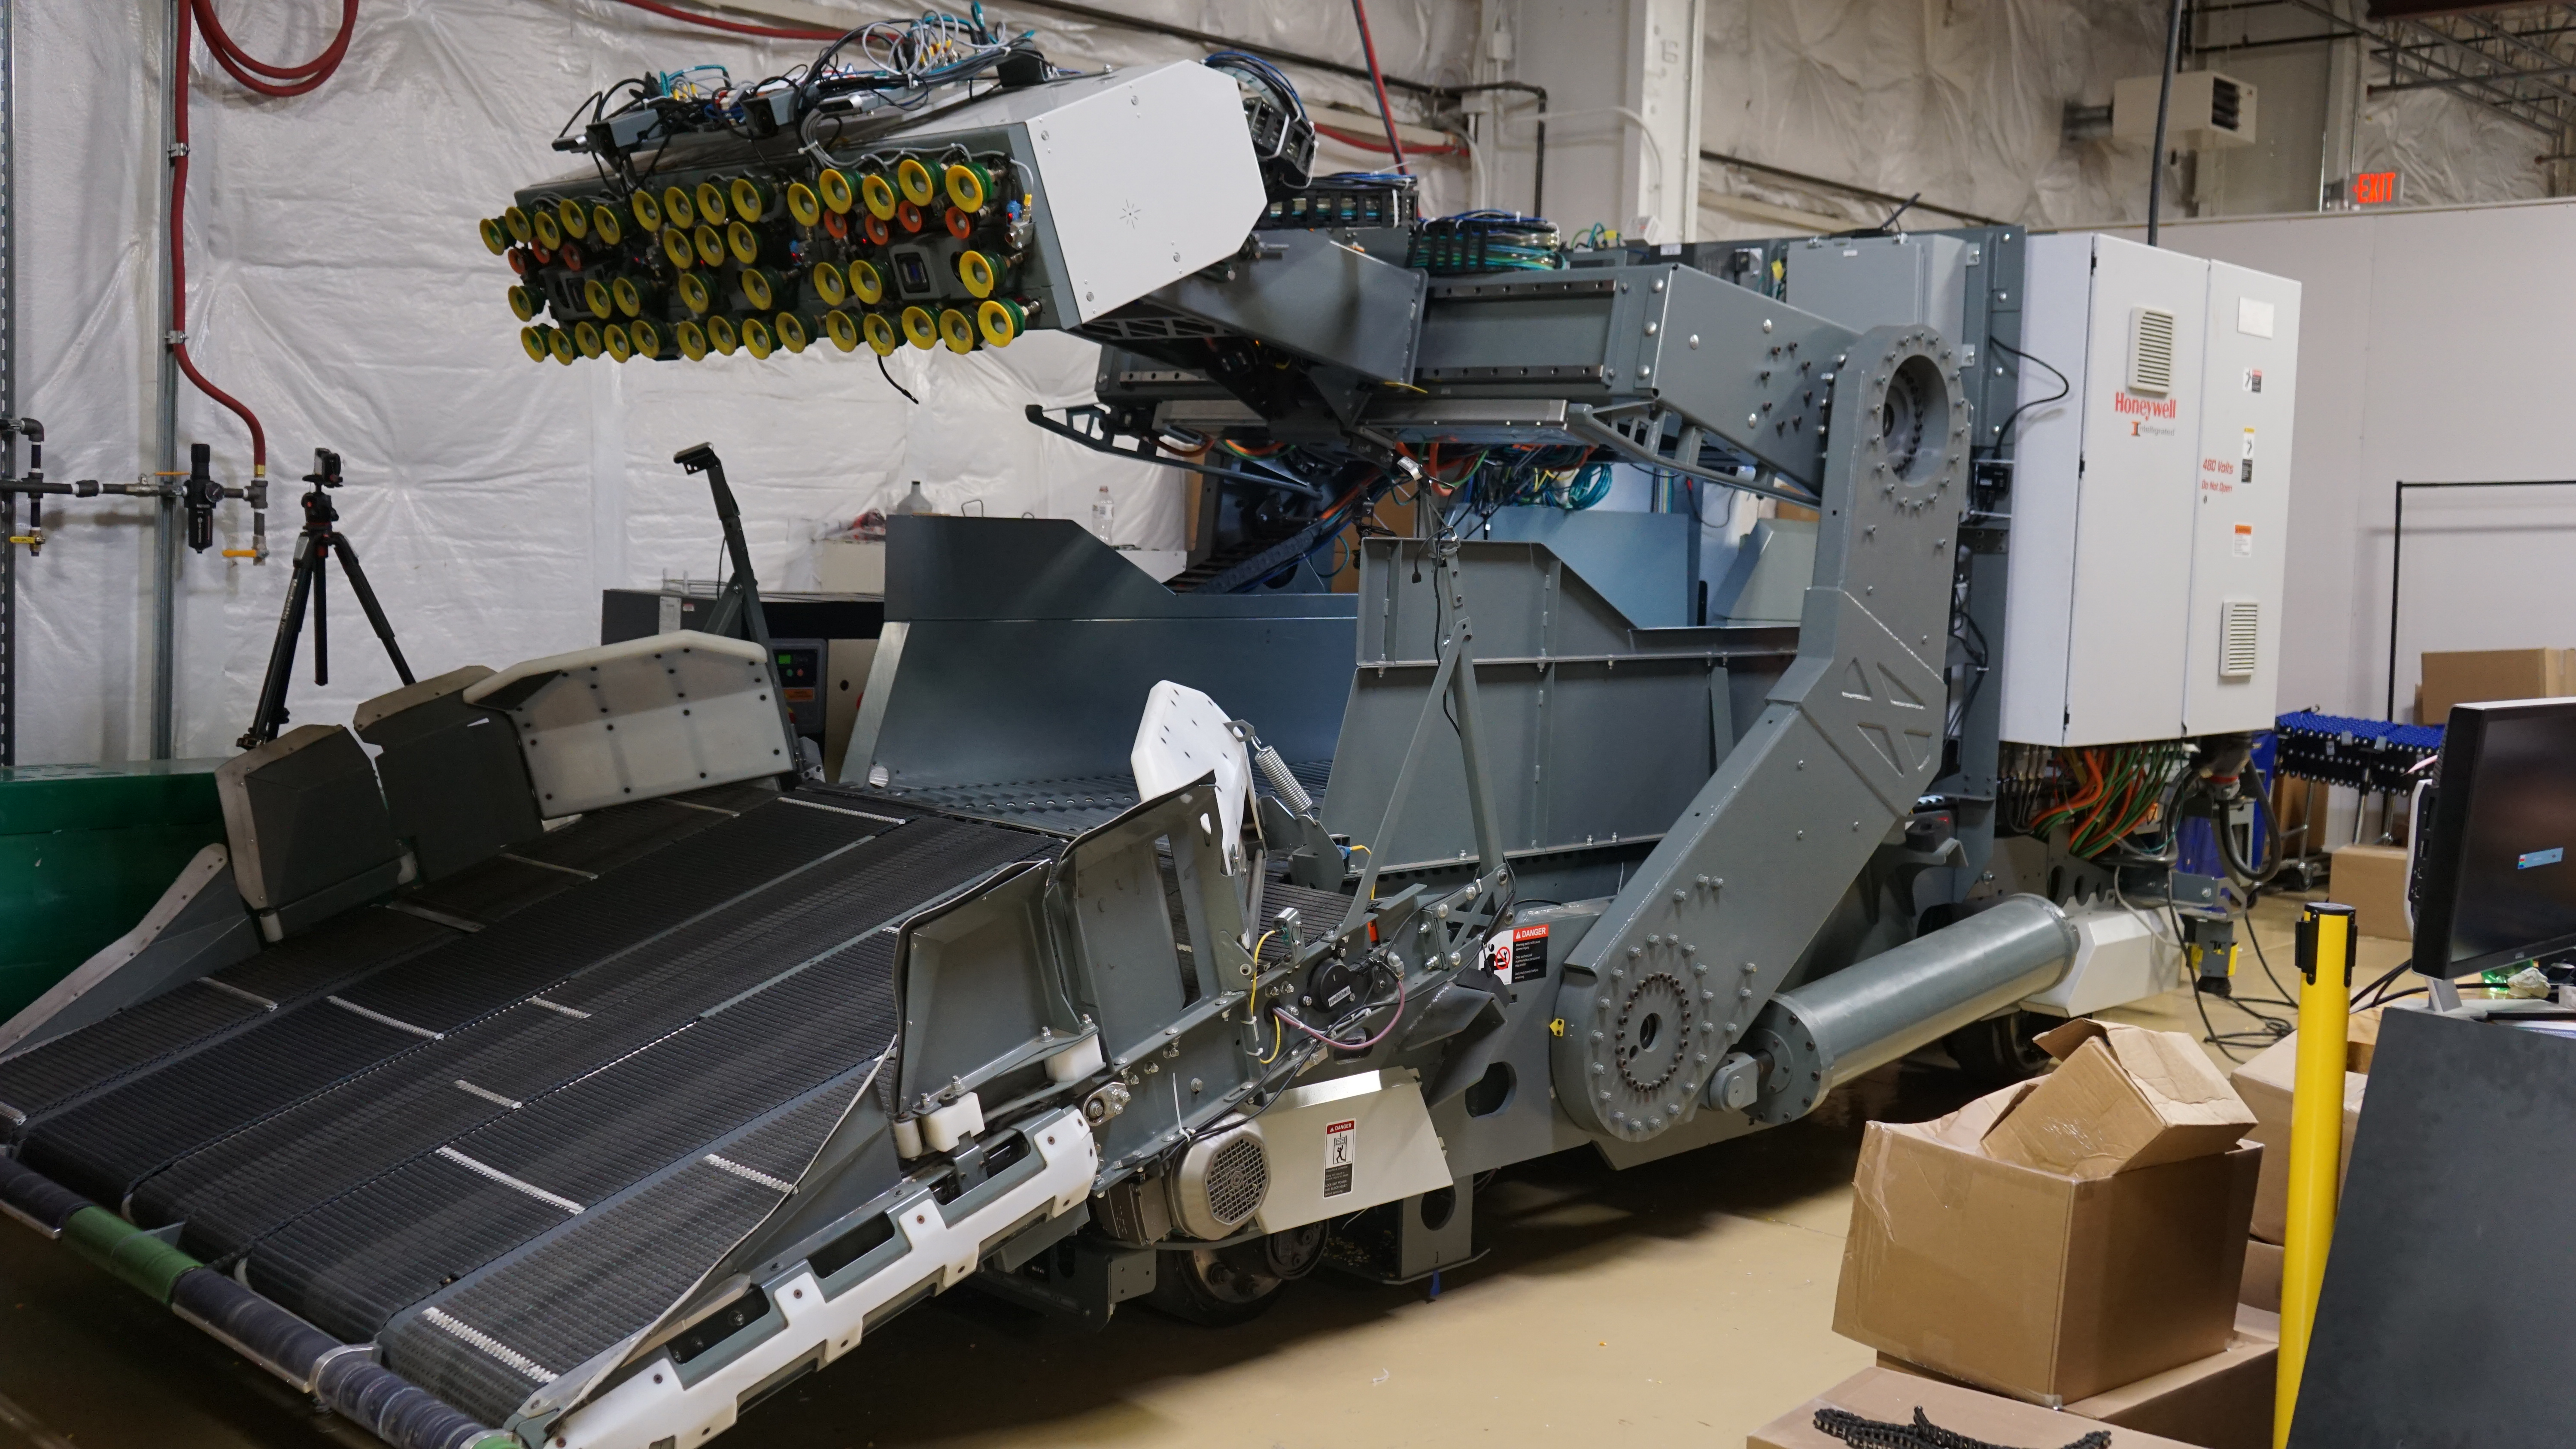
\includegraphics[width=0.6\textwidth]{gmt.pdf}
    % \vspace{-2mm}
  \caption{
  Truck-unloader robot with its manipulator-like (arm) and scooper-like (nose) end effectors
}
    \label{fig:gmt}
% \vspace{-6mm}
\end{figure}

\begin{figure}
\centering
\includegraphics[width=0.6\textwidth]{gmt_sim.png}
    % \vspace{-2mm}
  \caption{
  A simulated real world truck-unloading scenario
}
    \label{fig:gmt_sim}
% \vspace{-6mm}
\end{figure}

\begin{table*}[t]
\centering
     \resizebox{0.7\columnwidth}{!}{%
    % \resizebox{1.4\textwidth}{!}{\begin{minipage}{\textwidth}
        \begin{tabular}{ l | c c c c}  
           & arm & nose & arm+base & nose+base\\
         \hline
         WA* 		& 12.8 & 7.2 & 7.5 & 4.4 \\
         Our Method & 0.69 & 0.29 & 0.5 & 0.47 \\
        \end{tabular}
    }
    \caption{Comparison of mean planning times~[ms] averaged over 100 randomized queries for different modes of operation of the truck-unloading robot. The number of subregions preprocessed for each of these modes~(left to right) are~101,~7,~85 and~308.}
    \label{tab:gmt}
  % \end{center}
% \vspace{-6mm}
\end{table*}

As this algorithm is only applicable to static (known) environments, we only preprocessed it with collision checking against the walls of the truck and with self collision checking and not with the boxes inside the truck. We also tested our planner in a simulated real world scenario~(see Fig.\ref{fig:gmt_sim}) in conjunction with the WA* planner. For each query, we first ran our planner and validated the computed path against non-static obstacles i.e the boxes. We employed WA* as a fallback planner in case the first path is invalid. We observed that for all the queries ran for this scene, the fallback planner was never invoked. This experiment gave us an interesting use case for our planner to be employed in conjunction with conventional planners in the environments that are partially static.

\section{CTMP to Pickup Moving Objects off a Conveyor}
\label{sec:conveyor}
\subsection{Overview}
\subsection{Algorithmic Framework}
\subsubsection{Straw man Approach}
\subsubsection{Algorithm Building Blocks}
\subsubsection{Preprocessing Phase}
\subsubsection{Query Phase}
\subsection{Theoretical Analysis}
\subsubsection{Completeness}
\subsubsection{Time Complexity of Query Phase}
\subsection{Experimental Results}
\subsubsection{Experimental Setup}
\subsubsection{Real Robot Experiments}
\subsubsection{Simulation Experiments}

\section{Proposed Work}
\subsection{CTMP for Conveyor Task with Multiple Arms}
\subsection{CTMP for Motion Planning on Constrained Manifolds}
\subsection{Timeline}




\newpage

\bibliographystyle{IEEEtran}
\bibliography{references}

\end{document}
